\documentclass[a4paper,10pt]{article}
\usepackage[utf8]{inputenc}

%Preámbulos de las figuras

%--------------------------------------------
\usepackage{polynom}
%--------------------------------------------
\usepackage{nicematrix,tikz}
\usetikzlibrary{fit}
%--------------------------------------------
\usepackage[table, svgnames]{xcolor}
\usepackage{hhline, booktabs}
%--------------------------------------------
\usepackage{amsmath,gensymb}
\usetikzlibrary{matrix,positioning,calc}
\definecolor{COLOR1}{HTML}{6B99B9}
\definecolor{COLOR2}{HTML}{DD9CC4}
\tikzset{
    M/.style={
        matrix of math nodes,
        nodes={draw=none,anchor=center,minimum size=1.75em},
        nodes in empty cells,
    }
}
%Drawing code nesting in definition with parameters
\def\Det[color #1 size #2 line #3]#4#5{
    \draw[line width=#3,draw=#1, opacity=0.7]
    let \p1 = ($(#5)-(#4)$), % To access cartesian coordinates x, and y.
        \n2 = {atan2(\x1,\y1)}, % to get the angle of the line betwen #5 to #4
    in
    (#5.center)
        ++(90-\n2+90:#2/2)
        arc (90-\n2+90:90-\n2+90-180:#2/2)
        -- ($(#4.center)+(90-\n2-90:#2/2)$)
        arc (90-\n2-90:90-\n2-90-180:#2/2)
        -- cycle;
}
%--------------------------------------------
\usepackage{amssymb}
\newcommand{\ff}{\mathtt{f}}
%--------------------------------------------
\newcolumntype{A}{>{\columncolor{red!20}}c}
\newcolumntype{B}{>{\columncolor{blue!20}}c}

%%------------------------------------------------------------------------


\pagestyle{empty}
\begin{document}
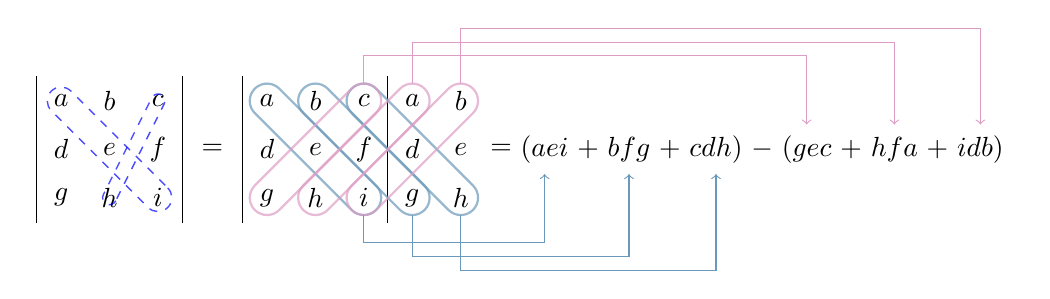
\begin{tikzpicture}
        \matrix[M] at (0,0) (M1){ % Matrix contents
            a & b & c  \\
            d & e & f  \\
            g & h & i  \\
        };

        \node[right=0em of M1](EQ){$=$};
        \matrix[M,right=0em of EQ](M2){ % Matrix contents
            a & b & c & a & b \\
            d & e & f & d & e \\
            g & h & i & g & h \\
        };
        \matrix[M,right=-1em of M2,column sep=-0.5em,](M3){ % Matrix contents
            = & (aei & + & bfg & + & cdh) & - & (gec & + & hfa & + & idb)\\
        };

        \foreach \a/\b/\c in {M1/1/west,M1/3/east,M2/1/west,M2/4/west}{\draw(\a-1-\b.north \c) -- (\a-3-\b.south \c);}
        \Det[color blue,dashed size 1em line 0.5pt]{M1-1-1}{M1-3-3} % test
        \Det[color blue,dashed size 0.5em line 0.5pt]{M1-1-3}{M1-3-2} %test
        \Det[color COLOR1 size 1.25em line 0.8pt]{M2-1-1}{M2-3-3}
        \Det[color COLOR1 size 1.25em line 0.8pt]{M2-1-2}{M2-3-4}
        \Det[color COLOR1 size 1.25em line 0.8pt]{M2-1-3}{M2-3-5}
        \Det[color COLOR2 size 1.25em line 0.8pt]{M2-3-1}{M2-1-3}
        \Det[color COLOR2 size 1.25em line 0.8pt]{M2-3-2}{M2-1-4}
        \Det[color COLOR2 size 1.25em line 0.8pt]{M2-3-3}{M2-1-5}
        \draw[COLOR1,->](M2-3-3)++(0,-1.25em/2)--++(0,-1em)-|(M3-1-2);
        \draw[COLOR1,->](M2-3-4)++(0,-1.25em/2)--++(0,-1.5em)-|(M3-1-4);
        \draw[COLOR1,->](M2-3-5)++(0,-1.25em/2)--++(0,-2em)-|(M3-1-6);
        \draw[COLOR2,->](M2-1-3)++(0,1.25em/2)--++(0,1em)-|(M3-1-8);
        \draw[COLOR2,->](M2-1-4)++(0,1.25em/2)--++(0,1.5em)-|(M3-1-10);
        \draw[COLOR2,->](M2-1-5)++(0,1.25em/2)--++(0,2em)-|(M3-1-12);
    \end{tikzpicture}
\end{document}